%
% teil3.tex -- Beispiel-File für Teil 3
%
% (c) 2020 Prof Dr Andreas Müller, Hochschule Rapperswil
%
% !TEX root = ../../buch.tex
% !TEX encoding = UTF-8
%
\subsection{Initialisierung
\label{buch:paper:varalg:subsection:initialization}}
\index{Initialisierung}%
Der Startpunkt eines genetischen Algorithmus ist die Initialisierung.
Dabei wird eine Population von zufälligen möglichen Lösungen erstellt.
Die Abbildung \ref{fig:possible_genetic_string} zeigt, wie eine mögliche
Lösung als genetischer String aussehen könnte.
\begin{figure}
	\centering
	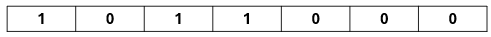
\includegraphics[width=0.8\textwidth]{
        papers/varalg/images/teil3/01GeneticString.png
        }
	\caption{
		Beispiel eines möglichen genetischen Strings, die 0 und 1 definieren dabei,
		ob die Funktion an dieser Position aktiviert ist oder nicht.
		}
	\label{fig:possible_genetic_string}
\end{figure}
Die Initialisierung besteht aus zwei Aspekten. Ein Aspekt ist die Grösse
der Population. Die Idee der begrenzten Grösse ist, dass nicht alle möglichen
Lösungen erstellt und überprüft werden müssen. Dies erspart Zeit und Ressourcen.
Der zweite Aspekt ist, dass die Permutationen alle zufällig erstellt werden.
Die zufällige Erzeugung der Anfangspopulation stellt ebenfalls eine Form 
der Variation dar. Sie sorgt dafür, dass die Suche nicht von einem begrenzten 
Bereich des Lösungsraums startet, sondern eine breite Palette von möglichen 
Lösungen berücksichtigt. Dabei werden jedoch keine Berechnungen durchgeführt,
die Hoffnung ist, dass durch die zufällige Erzeugung eine der Lösungen nahe
an das Optimum herankommt.

\subsubsection{Initialisierung auf das TSP angepasst
\label{buch:paper:varalg:subsection:initialization_tsp}}
In jeder Position kann ein Gen aktiviert (1) oder deaktiviert (0) sein.
Diese Logik eignet sich jedoch nicht für das
Travelling-Salesman-Problem, da eine Stadt nicht einfach
ein- oder ausgeschaltet werden kann.
Würde es auf alle möglichen Wege angewendet, müsste gewährleistet werden, 
dass nicht mehrere Wege aktiv sind. Die einfachste Logik ist, die Reihenfolge  
im String abzubilden. Dabei zeigt die Nummer der Stadt auf der jeweiligen Position
auf, ab wann diese besucht wird. Der Aufbau wäre wie in der 
Abbildung \ref{fig:cities_genetic_string} dargestellt.
\begin{figure}
	\centering
	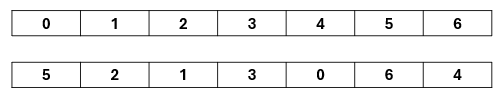
\includegraphics[width=0.8\textwidth]{
        papers/varalg/images/teil3/02GeneticStringCities.png
        }
	\caption{Beispiel von Städten in einem genetischen String dargestellt}
	\label{fig:cities_genetic_string}
\end{figure}
